\begin{frame}{Flamingo: Few-Shot Prompting with Images}
  \begin{itemize}\footnotesize\itemsep0.3em
    \item \textbf{Flamingo} (Alayrac et al., DeepMind, NeurIPS 2022) reads text interleaved with images or videos and writes text; CLIP-style dual encoders (covered earlier) only score image-text pairs.
    \item \textbf{Goal:} in-context learning (covered earlier) with images, as GPT-3, a 175B-parameter text-only language model, does with text. The prompt holds a few (image, text) examples and then the query image; the model completes the text, with no weight update.
    \item \textbf{Answers:} open-ended tasks such as captioning or visual question answering (VQA) use the generated text; multiple-choice tasks rank the candidates by their log-likelihood under the model.
  \end{itemize}
  \centering
  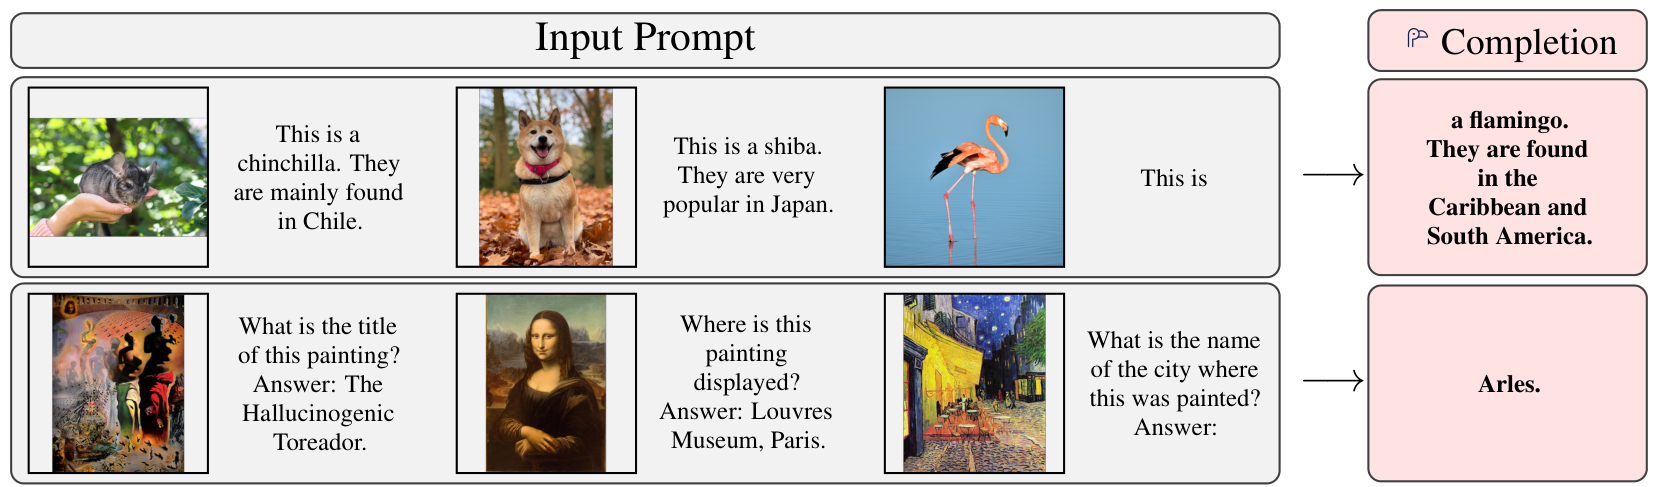
\includegraphics[width=\textwidth,height=0.36\textheight,keepaspectratio]{images/vision-language-models/flamingo_fig1_fewshot_prompts.png}\\[0.2em]
  {\scriptsize Two few-shot prompts and the completions of Flamingo-80B. Alayrac et al., ``Flamingo: a Visual Language Model for Few-Shot Learning,'' NeurIPS 2022, \href{https://arxiv.org/abs/2204.14198v2}{arXiv:2204.14198v2}, Figure~1 (first two rows).\par}
\end{frame}

\begin{frame}{Flamingo: Architecture}
  \begin{columns}[T,onlytextwidth]
    \column{0.56\textwidth}
      \centering
      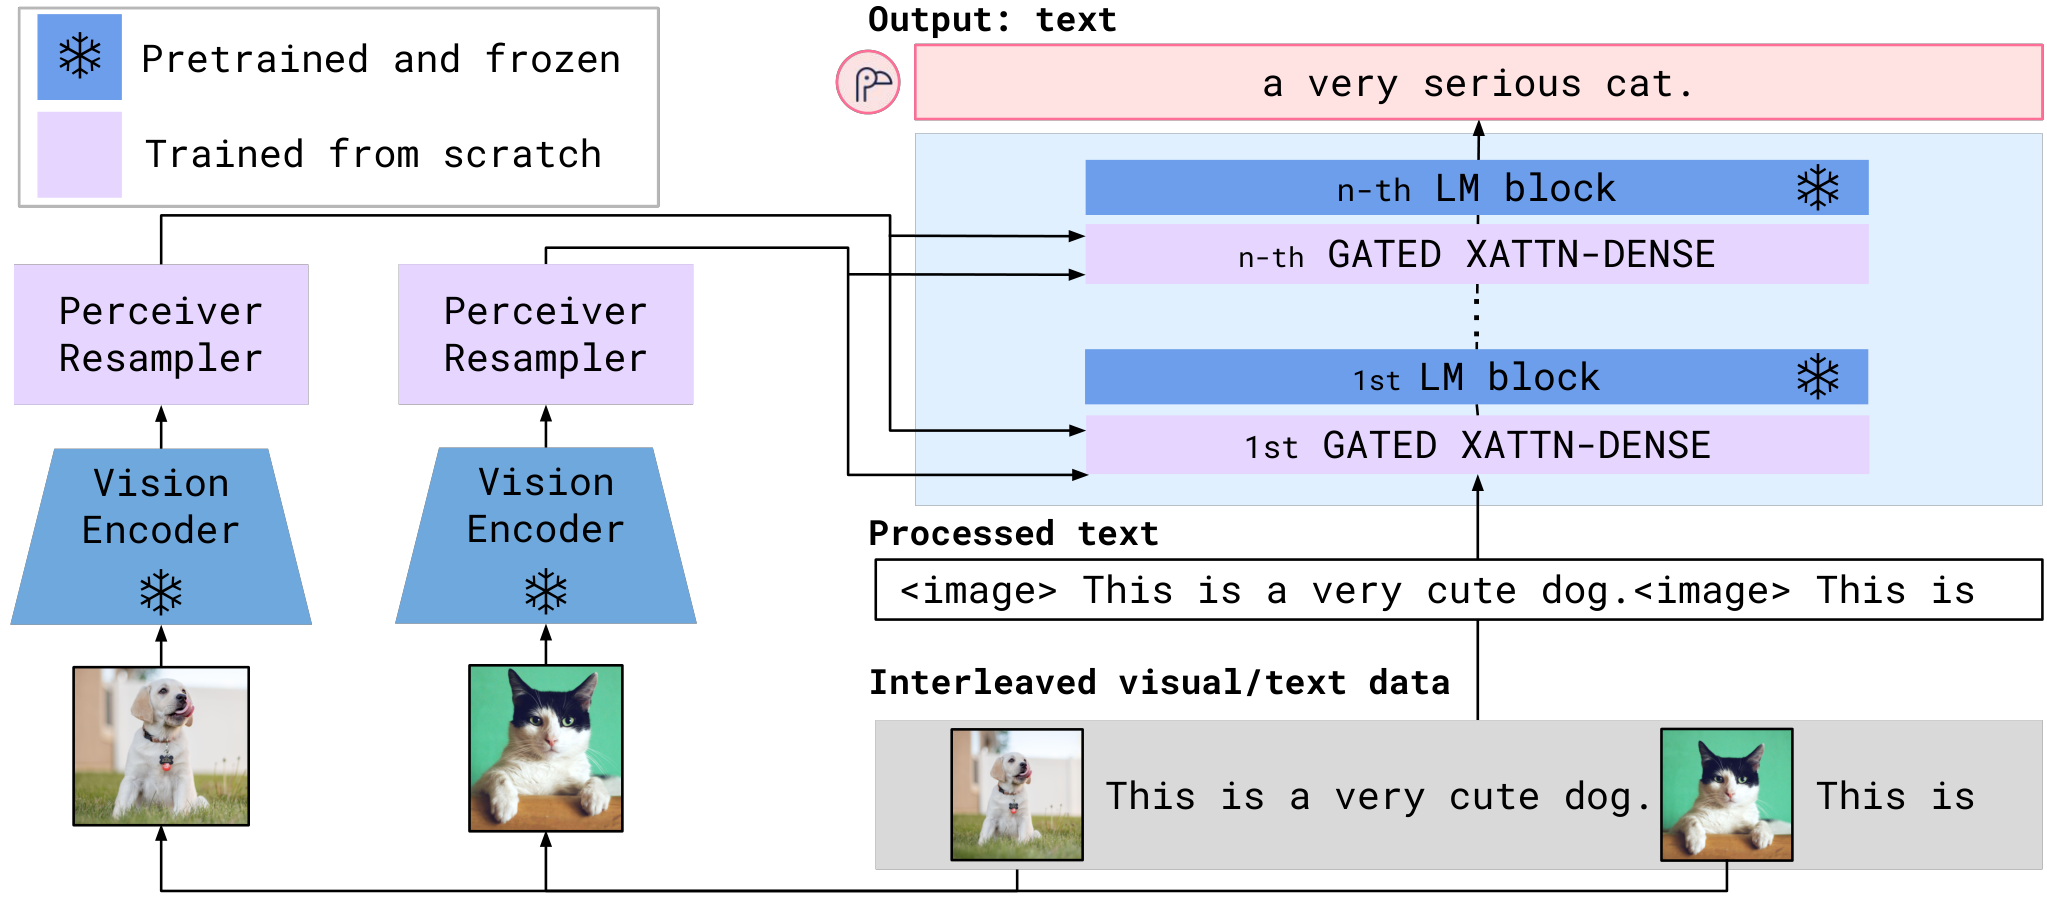
\includegraphics[width=\linewidth,height=0.46\textheight,keepaspectratio]{images/vision-language-models/flamingo_fig3_architecture.png}\\[0.2em]
      {\scriptsize Alayrac et al., \href{https://arxiv.org/abs/2204.14198v2}{arXiv:2204.14198v2}, Figure~3.\par}
    \column{0.42\textwidth}
      \begin{itemize}\footnotesize\itemsep0.3em
        \item \textbf{Frozen vision encoder:} NFNet-F6, a ResNet with no normalization layers, which the authors pretrained with CLIP's contrastive loss (covered earlier).
        \item \textbf{Frozen language model (LM):} Chinchilla, DeepMind's text-only LLM.
        \item \textbf{Trained from scratch:} the Perceiver Resampler and the GATED XATTN-DENSE layers (gated cross-attention plus a feed-forward layer) between frozen LM blocks.
      \end{itemize}
  \end{columns}
  \vspace{0.4em}
  {\centering\scriptsize
  \begin{tabular}{l l l r}
    \toprule
    \textbf{Model} & \textbf{Frozen LM} & \textbf{Trainable GATED XATTN-DENSE} & \textbf{Total} \\
    \midrule
    Flamingo-3B & 1.4B, 24 blocks & 1.2B: 24 layers, one before every LM block & 3.2B \\
    Flamingo-9B & 7.1B, 40 blocks & 1.6B: 10 layers, one before every 4th block & 9.3B \\
    Flamingo-80B & 70B, 80 blocks & 10B: 12 layers, one before every 7th block & 80B \\
    \bottomrule
  \end{tabular}\\[0.3em]
  All three also contain the frozen NFNet-F6 (435M parameters; Brock et al., ICML 2021) and a trainable Perceiver Resampler (194M); the LMs are Chinchilla models (Hoffmann et al., 2022). Alayrac et al., \href{https://arxiv.org/abs/2204.14198v2}{arXiv:2204.14198v2}, Tables~4 and~5.\par}
\end{frame}

\begin{frame}{Perceiver Resampler: A Fixed Number of Tokens}
  \begin{columns}[T,onlytextwidth]
    \column{0.58\textwidth}
      \begin{itemize}\footnotesize\itemsep0.25em
        \item \textbf{Input:} each frame's feature grid from the frozen encoder, plus a learned time embedding per frame, flattened into one sequence $X_f$ (an image is a one-frame video).
        \item \textbf{Latents:} 64 learned queries $X$ attend to keys and values $[X_f, X]$ (features and latents concatenated), then pass a feed-forward layer; 6 such layers.
        \item \textbf{Output:} always 64 visual tokens, whatever the image resolution or the number of video frames, so the LM's cross-attention cost does not grow with either.
        \item \textbf{Origin:} the Perceiver (Jaegle et al., ICML 2021) passes large inputs through a small learned latent array to avoid quadratic attention over the input. BLIP-2's Q-Former (earlier in this lecture) later used 32 such queries.
        \item \textbf{Ablation} (Flamingo-3B, 4 shots; score: each result as a percentage of the state of the art, averaged over five benchmarks): Resampler 70.7; MLP 66.6 and plain Transformer 66.7, both slower.
      \end{itemize}
    \column{0.40\textwidth}
      \centering
      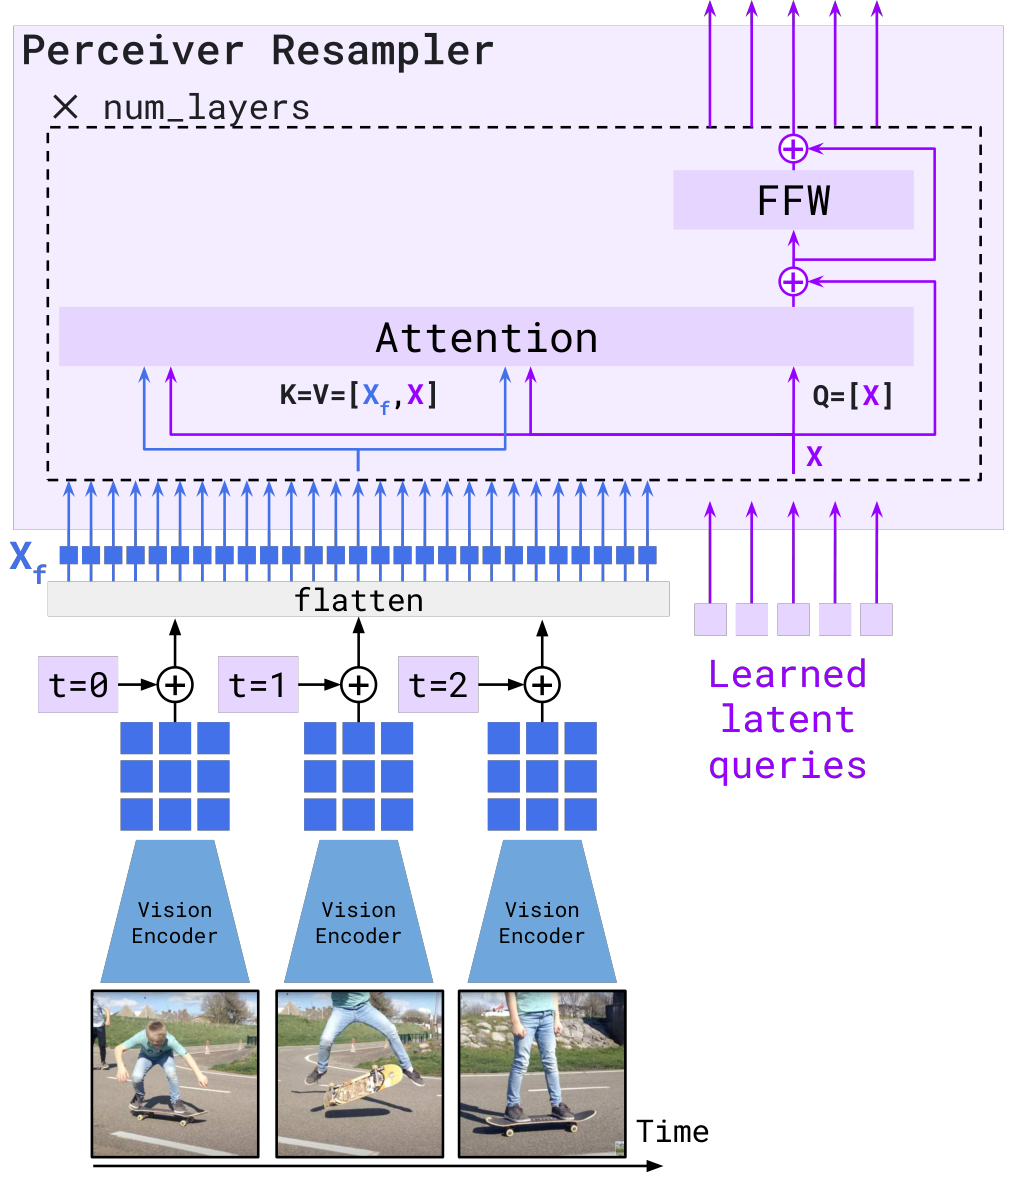
\includegraphics[width=\linewidth,height=0.64\textheight,keepaspectratio]{images/vision-language-models/flamingo_fig5_perceiver_resampler.png}\\[0.2em]
      {\scriptsize The figure draws a three-frame video and five output tokens; the model outputs 64. Alayrac et al., \href{https://arxiv.org/abs/2204.14198v2}{arXiv:2204.14198v2}, Figure~5 (pseudo-code omitted); ablation: Table~3.\par}
  \end{columns}
\end{frame}

\begin{frame}{Gated Cross-Attention Starts as the Frozen LM}
  \begin{columns}[T,onlytextwidth]
    \column{0.62\textwidth}
      {\footnotesize Each GATED XATTN-DENSE block updates the language features $y$ with the visual tokens $x$, then passes $y$ to the next frozen LM block:
      \[ \begin{aligned}
        y &\leftarrow y + \tanh(\alpha_{\mathrm{xattn}})\cdot \mathrm{Attn}(q{=}y,\ kv{=}x)\\
        y &\leftarrow y + \tanh(\alpha_{\mathrm{dense}})\cdot \mathrm{FFW}(y)
      \end{aligned} \]
      $\alpha_{\mathrm{xattn}}$, $\alpha_{\mathrm{dense}}$: learnable scalars of the block, initialized to 0; Attn: attention with queries from $y$, keys and values from $x$; FFW: feed-forward layer.\par}
      \begin{itemize}\footnotesize\itemsep0.3em
        \item \textbf{At initialization} $\tanh(0)=0$, so the new branches add nothing and the model computes exactly the pretrained LM; the authors report better training stability and final performance.
        \item \textbf{Ablations} (score 70.7): no tanh gate 66.5, with unstable training; vanilla Transformer-decoder cross-attention 66.9; layers stacked on top of the unchanged LM 63.1.
        \item \textbf{Freezing the LM} prevents catastrophic forgetting of what pretraining taught: fine-tuning the LM scores 62.7, training it from scratch 57.8.
      \end{itemize}
    \column{0.36\textwidth}
      \centering
      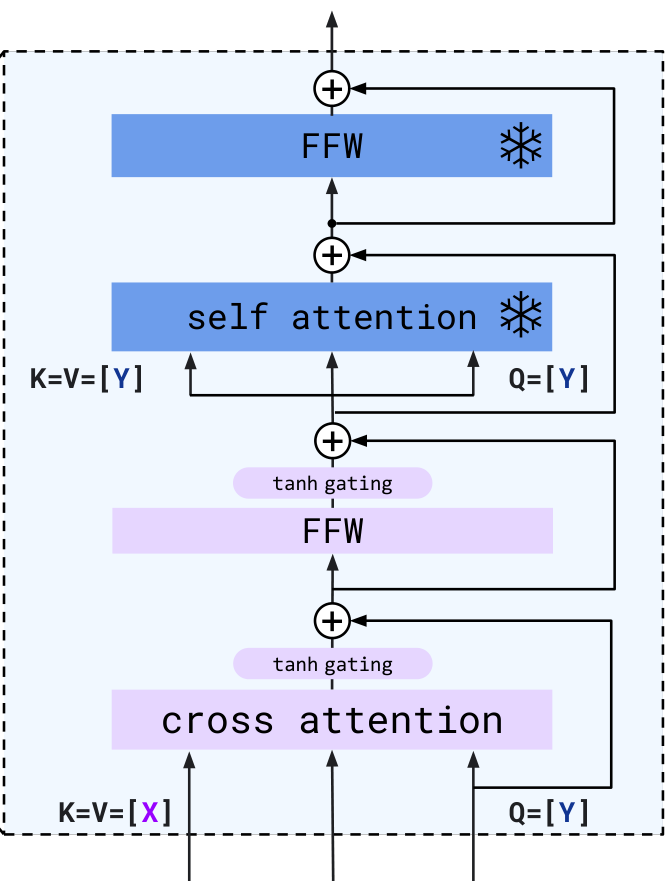
\includegraphics[width=\linewidth,height=0.62\textheight,keepaspectratio]{images/vision-language-models/flamingo_fig4_gated_xattn_dense.png}\\[0.2em]
      {\scriptsize One GATED XATTN-DENSE block (purple, trained) feeding a frozen LM block (blue). Alayrac et al., \href{https://arxiv.org/abs/2204.14198v2}{arXiv:2204.14198v2}, Figure~4 (middle panel); ablations: Table~3.\par}
  \end{columns}
\end{frame}

\begin{frame}{Interleaved Inputs and Per-Image Masking}
  \begin{itemize}\footnotesize\itemsep0.3em
    \item \textbf{One text stream:} a web page or a few-shot prompt becomes text with an \texttt{<image>} tag at each image's position. A learned \texttt{<EOC>} (end of chunk) token closes the text before each image and at the end; \texttt{<BOS>} (beginning of sequence) starts it.
    \item \textbf{Per-image attention masking:} let $\phi(\ell)$ be the index of the last image before text position $\ell$ (0 if none). Token $\ell$ cross-attends only to the visual tokens of image $\phi(\ell)$; all others are masked.
  \end{itemize}
  {\centering\scriptsize
  \begin{tabular}{l c c c}
    \toprule
    \textbf{Text chunk} & $\phi(\ell)$ & \textbf{Image 1 tokens} & \textbf{Image 2 tokens} \\
    \midrule
    \texttt{<BOS>Cute pics of my pets!<EOC>} & 0 & masked & masked \\
    \texttt{<image>My puppy sitting in the grass.<EOC>} & 1 & visible & masked \\
    \texttt{<image>My cat looking very dignified.<EOC>} & 2 & masked & visible \\
    \bottomrule
  \end{tabular}\\[0.3em]
  Example and mask after Alayrac et al., \href{https://arxiv.org/abs/2204.14198v2}{arXiv:2204.14198v2}, Figure~7, with one row per chunk where the paper draws one per token; $\phi$ from Appendix~A.1.3, ablation from Table~10.\par}
  \begin{itemize}\footnotesize\itemsep0.3em
    \item \textbf{Earlier images still count:} the frozen LM's causal self-attention reads every earlier text token, and those tokens have already attended to their own image. Trained on sequences of at most 5 images, the model still benefits from prompts with up to 32 (image, text) shots.
    \item \textbf{Ablation:} cross-attending to all previous images lowers the score from 70.7 to 63.5. In training, a random half of the web pages map text to the next image instead (App.~A.3.2).
  \end{itemize}
\end{frame}

\begin{frame}{Flamingo: Training Data and Objective}

  {\centering\scriptsize
  \begin{tabular}{l p{8.3cm} l c}
    \toprule
    \textbf{Dataset} & \textbf{Content} & \textbf{Size} & $\lambda_m$ \\
    \midrule
    M3W & MultiModal MassiveWeb: web pages with their images kept in place & about 43M pages & 1.0 \\
    ALIGN & images with their alt-text (earlier in this lecture) & 1.8B pairs & 0.2 \\
    LTIP & Long Text \& Image Pairs: 20.5-token captions on average (ALIGN: 12.4) & 312M pairs & 0.2 \\
    VTP & Video \& Text Pairs: short videos (about 22\,s) with one sentence each & 27M videos & 0.03 \\
    \bottomrule
  \end{tabular}\par}
  \begin{itemize}\footnotesize\itemsep0.3em
    \item \textbf{Objective:} a weighted sum of per-dataset negative log-likelihoods of the text given the preceding images; the gradients of all $M=4$ datasets are summed at every step.
    \[ \sum_{m=1}^{M} \lambda_m\, \mathbb{E}_{(x,y)\sim\mathcal{D}_m}\Big[-\sum_{\ell=1}^{L}\log p\big(y_\ell \mid y_{<\ell},\, x_{\leq\ell}\big)\Big] \]
    $\mathcal{D}_m$: dataset $m$, with weight $\lambda_m$; $y_\ell$: the $\ell$-th of $L$ text tokens; $y_{<\ell}$: the tokens before it; $x_{\leq\ell}=\{x_i : i\leq\phi(\ell)\}$: the images before it.
    \item \textbf{Web data only}, none annotated for machine learning; pairs are written as \texttt{<image>}caption\texttt{<EOC>} to match M3W. The paper ties the few-shot ability to M3W: without it the score falls from 70.7 to 53.4 (without the image-text pairs: 60.9; round-robin updates in place of summed gradients: 62.9).
  \end{itemize}
  \vspace{0.1em}
  {\scriptsize Alayrac et al., \href{https://arxiv.org/abs/2204.14198v2}{arXiv:2204.14198v2}, Section~2.4, Appendices~A.3.3 and~B.1.2, Table~3.\par}
\end{frame}

\begin{frame}{Flamingo: Results and Legacy}
  \centering
  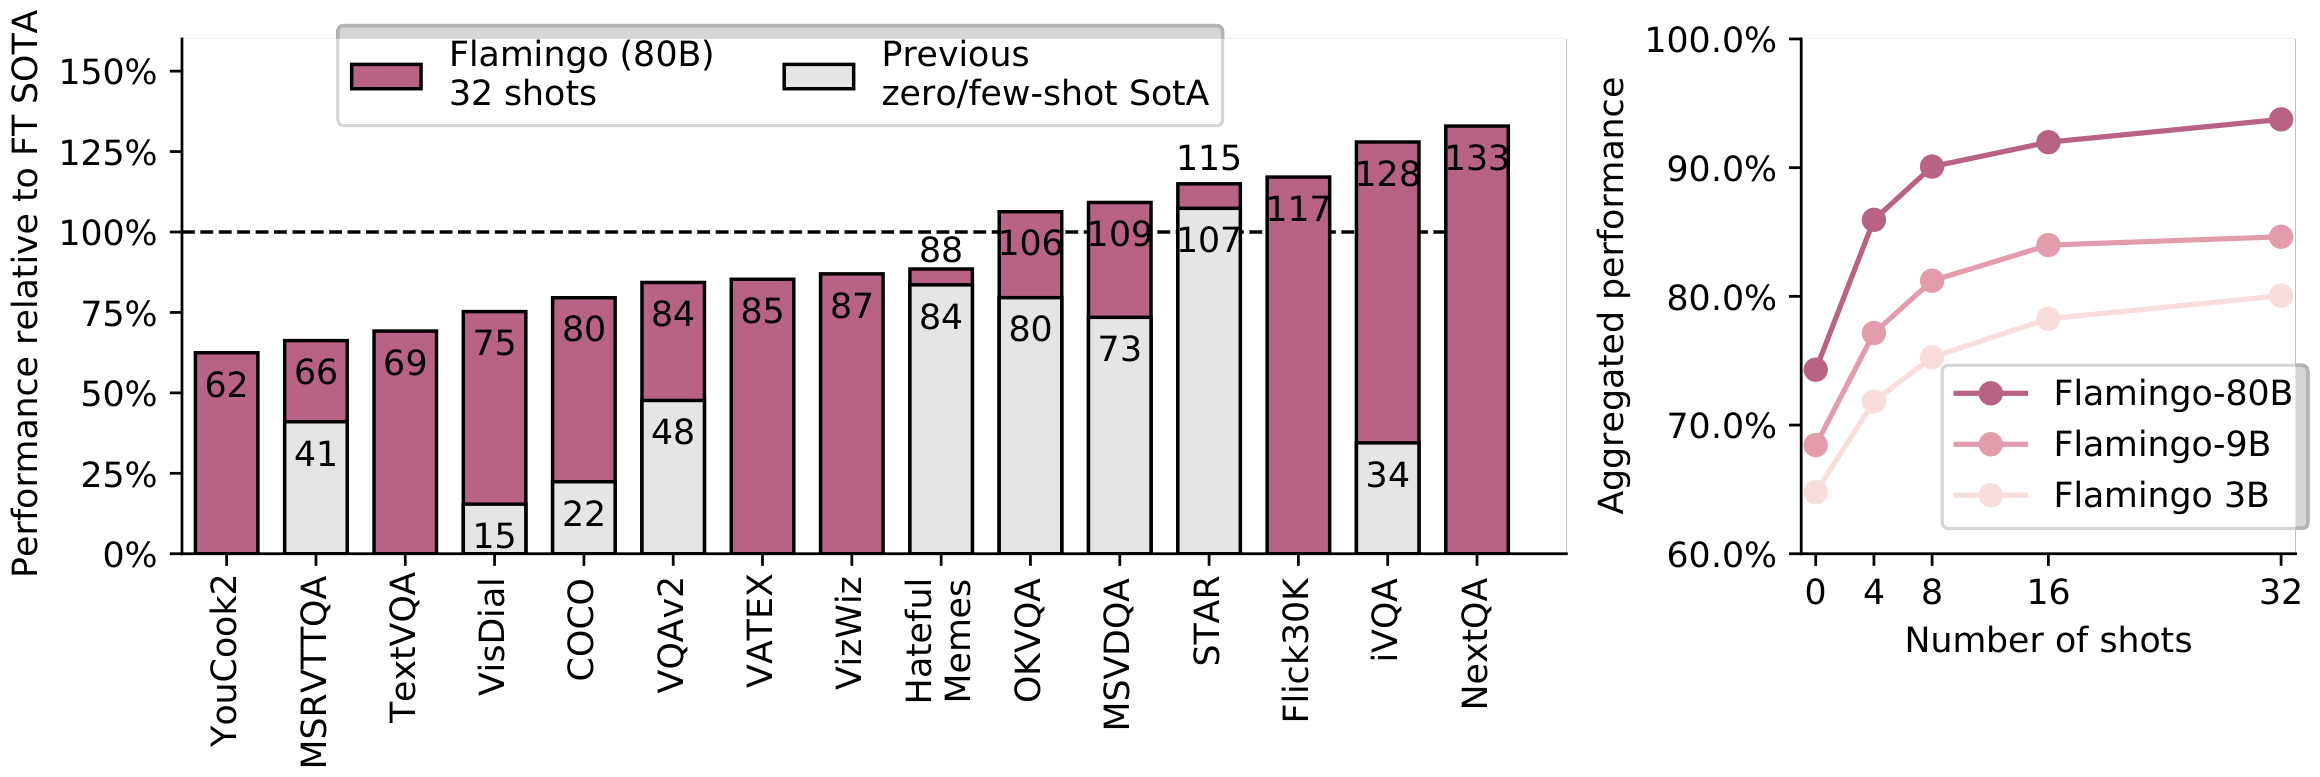
\includegraphics[width=\textwidth,height=0.34\textheight,keepaspectratio]{images/vision-language-models/flamingo_fig2_results_overview.png}\\[0.2em]
  {\scriptsize Right: performance rises with shots and model size. Alayrac et al., \href{https://arxiv.org/abs/2204.14198v2}{arXiv:2204.14198v2}, Figure~2, Section~1.\par}
  \raggedright
  \begin{itemize}\footnotesize\itemsep0.3em
    \item \textbf{Results:} one set of weights, 16 benchmarks. With 32 shots Flamingo-80B beats the fine-tuned state of the art on 6 (bars above the dashed line), using about 1000 times less task-specific data.
    \item \textbf{Open versions:} OpenFlamingo (Awadalla et al., 2023), five 3B to 9B models averaging 80--89\% of the matching Flamingo on seven datasets; IDEFICS (9B, 80B), trained with OBELICS (141M open web pages, 353M images; Lauren\c{c}on et al., 2023), is often on par with Flamingo.
    \item \textbf{Still in use:} cross-attention layers inside a frozen LLM, as in Flamingo, are one of the two ways of adding vision compared later in this lecture.
  \end{itemize}
  {\scriptsize Sources: Awadalla et al., ``OpenFlamingo: An Open-Source Framework for Training Large Autoregressive Vision-Language Models,'' 2023, \href{https://arxiv.org/abs/2308.01390v2}{arXiv:2308.01390v2}; Lauren\c{c}on et al., ``OBELICS: An Open Web-Scale Filtered Dataset of Interleaved Image-Text Documents,'' 2023, \href{https://arxiv.org/abs/2306.16527v2}{arXiv:2306.16527v2}.\par}
\end{frame}
